\documentclass[12pt,letterpaper]{article}
\usepackage{fullpage}
\usepackage[top=2cm, bottom=4.5cm, left=2.5cm, right=2.5cm]{geometry}
\usepackage{amsmath,amsthm,amsfonts,amssymb,amscd}
\usepackage{lastpage}
\usepackage{enumerate}
\usepackage{fancyhdr}
\usepackage{mathrsfs}
\usepackage{xcolor}
\usepackage{graphicx}
\usepackage{listings}
\usepackage{hyperref}
\usepackage[T1]{fontenc}
\usepackage{textcomp}

\hypersetup{
  colorlinks=true,
  linkcolor=blue,
  linkbordercolor={0 0 1}
}

\definecolor{limitblue}{RGB}{32, 76, 113}
\definecolor{ruddybrown}{rgb}{0.73, 0.4, 0.16}
\colorlet{punct}{red!60!black} 
\definecolor{background}{HTML}{EEEEEE}
\definecolor{delim}{RGB}{20,105,176}
\definecolor{ogreen}{rgb}{0.0, 0.5, 0.0}
\colorlet{numb}{magenta!60!black}
 
\renewcommand\lstlistingname{Code}
\renewcommand\lstlistlistingname{Codes}
\def\lstlistingautorefname{Alg.}

\lstdefinestyle{Python}{
  language        = Python,
  frame           = lines, 
  basicstyle      = \footnotesize,
  keywordstyle    = \color{blue},
  stringstyle     = \color{green},
  commentstyle    = \color{red}\ttfamily
}
\lstdefinestyle{R}{
  language        = R,
  frame           = lines,
  captionpos      = b,
  abovecaptionskip= 10pt, 
  emphstyle       = \textbf,
  framextopmargin = 4pt,
  framexbottommargin = 4pt,
  basicstyle      = \ttfamily\footnotesize,
  keywordstyle    = \color{limitblue},
  stringstyle     = \color{ruddybrown},
  showstringspaces= false,
  commentstyle    = \color{red}\ttfamily,
  tabsize         = 2,
  literate=
    *{0}{{{\color{numb}0}}}{1}
      {1}{{{\color{numb}1}}}{1}
      {2}{{{\color{numb}2}}}{1}
      {3}{{{\color{numb}3}}}{1}
      {4}{{{\color{numb}4}}}{1}
      {5}{{{\color{numb}5}}}{1}
      {6}{{{\color{numb}6}}}{1}
      {7}{{{\color{numb}7}}}{1}
      {8}{{{\color{numb}8}}}{1}
      {9}{{{\color{numb}9}}}{1}
      {:}{{{\color{punct}{:}}}}{1}
      {,}{{{\color{punct}{,}}}}{1}
      {\{}{{{\color{delim}{\{}}}}{1}
      {\}}{{{\color{delim}{\}}}}}{1}
      {[}{{{\color{delim}{[}}}}{1}
      {]}{{{\color{delim}{]}}}}{1}
}

\setlength{\parindent}{0.0in}
\setlength{\parskip}{0.05in}

% Edit these as appropriate
\newcommand\course{Statistics I}
\newcommand\hwnumber{10.2}                  % <-- homework number
\newcommand\NetIDa{Atreya Choudhury}           % <-- NetID of person #1
\newcommand\NetIDb{bmat2005}           % <-- NetID of person #2 (Comment this line out for problem sets)

\pagestyle{fancyplain}
\headheight 35pt
\lhead{\NetIDa}
\lhead{\NetIDa\\\NetIDb}                 % <-- Comment this line out for problem sets (make sure you are person #1)
\chead{\textbf{\Large Assignment \hwnumber}}
\rhead{\course \\ \today}
\lfoot{}
\cfoot{}
\rfoot{\small\thepage}
\headsep 2em

\begin{document}
\textit{A marketing analyst is studying the relationship between x = money spent on television advertising and y = increase in sales. One study reported the following data (in dollars) for a a particular company.}
\begin{center}
  \begin{tabular}{ c|cccccccccc }
    \hline
    x & 380 & 645 & 360 & 900 & 540 & 670 & 820 & 1050 & 760 & 800\\
    \hline
    y & 550 & 780 & 530 & 1200 & 620 & 800 & 910 & 1400 & 830 & 905\\
    \hline
  \end{tabular}
\end{center}

\begin{enumerate}[a.] \setlength{\itemsep}{30pt}
  \item Develop a scatterplot and determine whether a linear relationship appear to provide a good fit to this data set.
  
  \textbf{Solution:}
  \begin{figure*}[h]
    \centering
    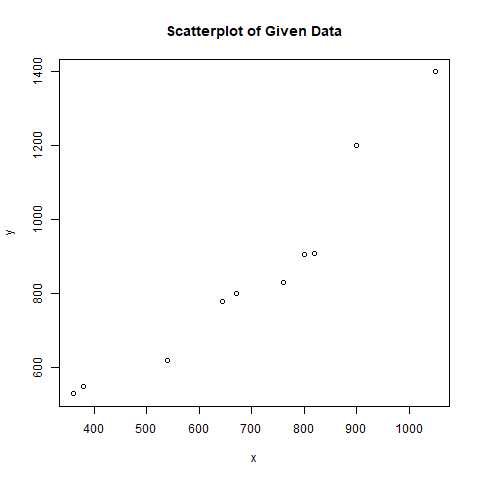
\includegraphics[width=12cm]{Scatterplot.png}
    \caption{Scatterplot}
  \end{figure*}
  The plot shows that there can be a linear relationship between y and x.
  \newpage
  \item What is the least squares regression equation?

  \textbf{Solution:}
  Using lm() on the plot gives 27.543 as the intercept and 1.191 as the value of x.
  The least squares regression equation is given
  $$y = 1.191x + 27.543$$
  \begin{figure*}[h]
    \centering
    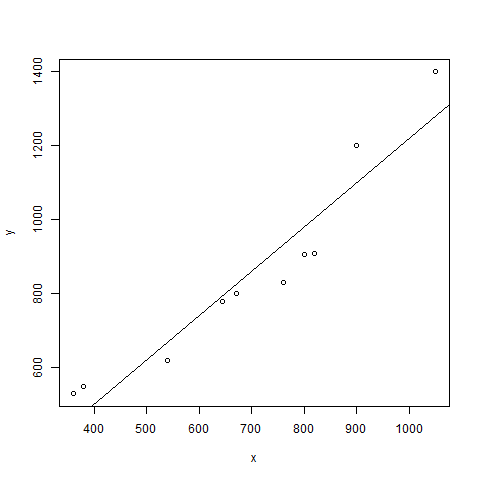
\includegraphics[width=12cm]{ScatterplotWithRegression.png}
    \caption{Linear Model}
  \end{figure*}
  \item Interpret the estimated slope and y intercept for this problem.

  \textbf{Solution:}
  The slope is positive which indicates that the increment in sales increases with increase in money spent on advertising.
  The positive intercept indicates that the company can expect an increase in sales even without investing any money on advertising. 
  \item What are the values of $s^2$ and the sum of squares for error (SSE)?

  \textbf{Solution:}
  $s^2$ = 7980.648\\
  SSE = 63845.10
  \item Find and interpret the correlation coefficient.

  \textbf{Solution:}
  The correlation coefficient is equal to 0.9522339.

  The coefficient is positive which indicates that the data is positively correlated. Also, it is close to 1. This indicates that the linear model is accurate.
  \item Find and interpret the coefficient of determination.

  \textbf{Solution:}
  The coefficient of determination is equal to 0.9067494.

  It is close to 1. This indicates that the linear model is accurate.
  \item Construct a 95\% confidence interval for the slope.

  \textbf{Solution:}
  95\% confidence interval of the slope is (0.8798089, 1.502738).
  \item Conclude from the above if the slope can be one.

  \textbf{Solution:}
  As 1 lies in the confidence interval, there is a 95\% chance that the slope is 1.
\end{enumerate}
\newpage
\lstinputlisting[language=R, style=R, title=R Code]{code.R}
\end{document}